\section{Linkages}
\begin{figure}[h]
 \begin{center}
  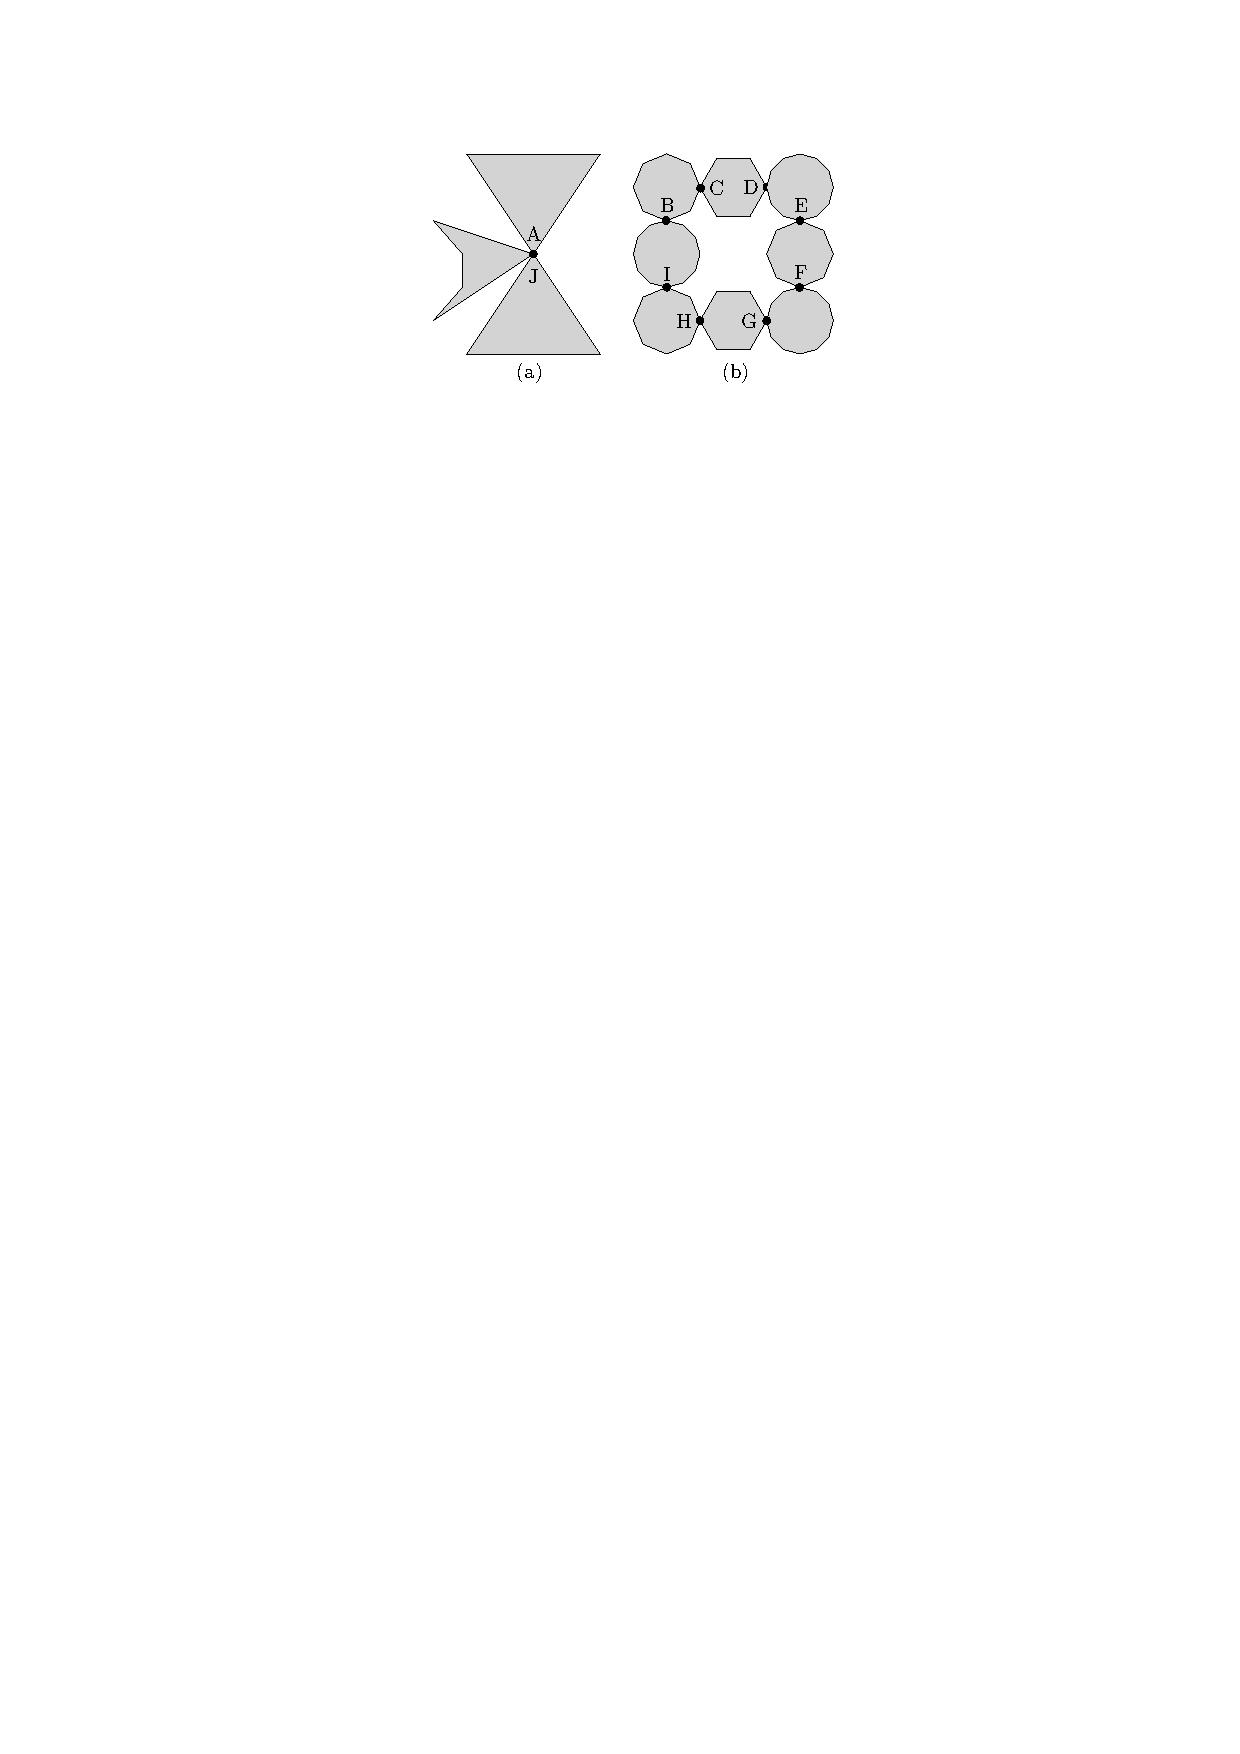
\includegraphics[scale=1]{graphics/linkageillustration.pdf}
  \caption{An embedded linkage}
 \end{center}

\end{figure}

%graph -> G = (V,E)
%linkage -> (G,l)
%embedding -> 
When graphs model physical objects, distances between adjacent vertices matter. The length 
assignment of a graph $G=(V,E)$ is $\ell:E \mapsto \bbr^+$. A \textit{linkage} is a graph $G = 
(V,E)$ with a length assignment $l:E \mapsto \bbr^+$.  
%Inser linkage here

We consider embeddings of a graph that 
respects the length assignment.  A \textit{realization} of a linkage, $G$ and $l$, is an embedding 
of a graph, $\Pi$, such that for every edge $\{u,v\} \in E$, $\ell\left( \{u,v\} \right) 
= \left\vert \Pi(u) - \Pi(v) \right\vert$.  A \textit{plane realization} is a 
plane embedding with the property, $l\left( \{u,v\} \right) 
= \left\vert \Pi(u) - \Pi(v) \right\vert$.

%(fig 1) insert a table of a graph and define a length assigment 
%(fig 2) insert a realization of (fig 1)
%(fig 3) insert a second realization of (fig 1)



%graph component of the linkage   the plane.  A linkage 
%\textit{embedding} is $L : V \mapsto 
%\bbR^{2}$.
% A \textit{linkage} is an ordered pair $G = (V,E)$ comprising of a set $V$ of vertices or nodes 
% together with a set $E$ of edges or lines. This definition is commonly used for graphs.  Mapping 
% the linkage $G$ into the plane is said to be the \textit{embedding}, i.e. $L : V \mapsto 
% \bbR^{2}$.  A length function correspond to a linkage, $l: E \mapsto \bbr^+$ gives a length to an 
% edge in the linkage.  If We consider a \textit{realization} of a linkage is range of $L$, i.e. 
% $L(V)$. If for every edge $(u,v) \in E$ such that $l\left( \left(u,v\right) \right) = \left\vert 
% L(u) - L(v) \right\vert$ is true, then $L$ is said to be a \textit{proper embedding} of $G$.
% \begin{figure}[h]
% \begin{center}
% 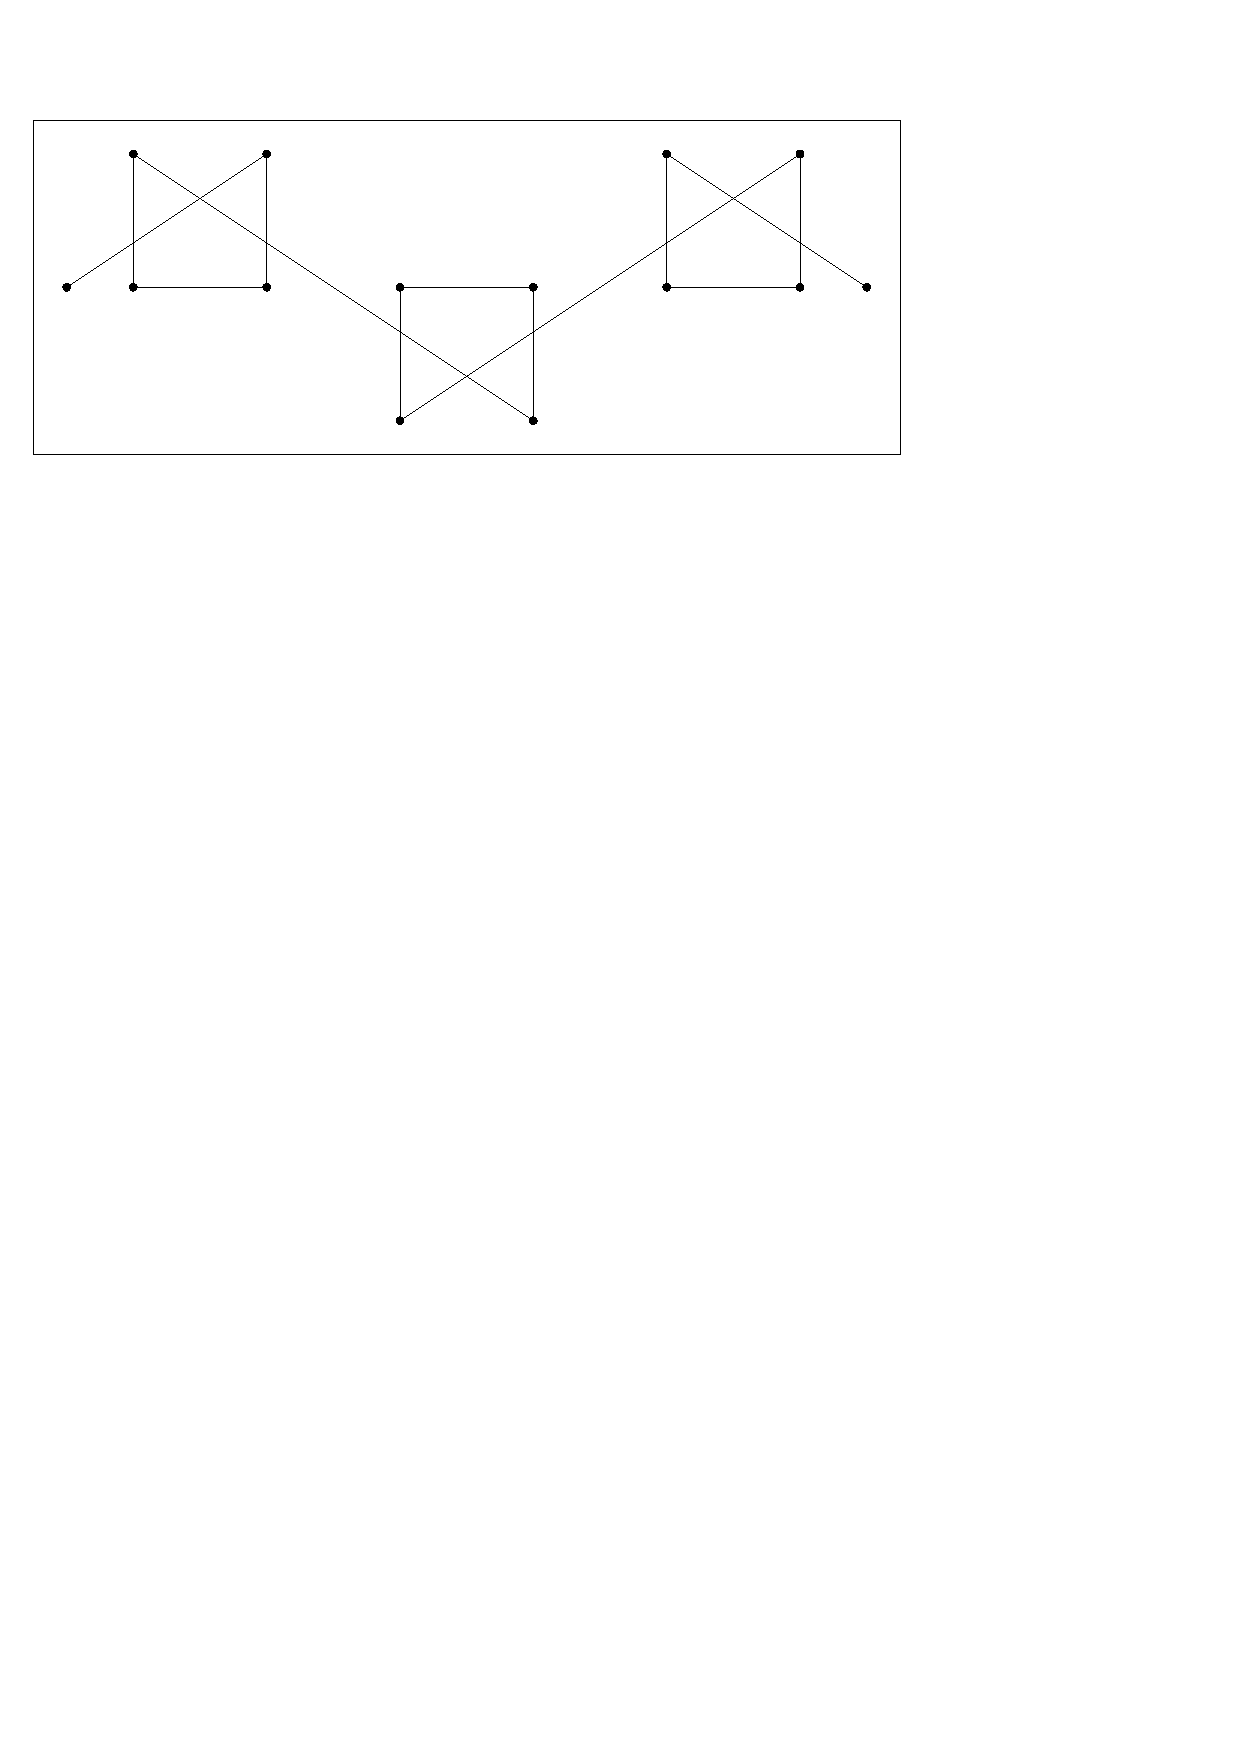
\includegraphics[scale=1]{graphics/crossingEdgeLinkage.pdf}
% \end{center} 
% \caption{A linkage where edges cross however it does not contain loops or multiple edges between 
% vertices.}
% \label{fig:linkage-3}
% \end{figure}
